\chapter[Algebraic approaches to quantum-gravity regimes]{Algebraic approaches to\\ quantum-gravity regimes}

Chapters~6--8 analyzed an existing structure — AdS/CFT — using the machinery built in Chapters~2--5. This
chapter does something different and, in a sense, more ambitious: it builds simple, completely solvable
\emph{toy models} of quantum gravity directly out of operator algebras, with the crossed product of Chapter~5
appearing not as an abstract mathematical device but as the literal, physical mechanism that turns a quantum
field theory's type $\mathrm{III}_1$ algebra into the finite, well-defined entropy of a black hole or of
de~Sitter space. This is the payoff the whole crossed-product construction was built for.

\section{A model of gravitational dressing from observers}

\subsection*{Setting up the constraint}

Start with an ordinary quantum field theory on Hilbert space $\HH_Q$, and let $\M$ be the algebra of some
region, $\M'$ its commutant, both type $\mathrm{III}_1$, with a cyclic-separating reference $\ket\Psi$ and
modular Hamiltonian $K$ generating the usual internal time flow on $\M$ and $\M'$ (Chapter~4).

Now attach two observers, $R$ and $L$, each with their own Hamiltonian $\hat q_R,\hat q_L$ and conjugate
clock-reading operators $\hat p_R,\hat p_L$ (with clock-reading eigenstates $\ket\tau_R,\ket\tau_L$). Demand
the \emph{whole} system — field theory plus both observers — be invariant under translations generated by
\[
H = K + \hat q_R - \hat q_L .
\]
This is a toy \textbf{Hamiltonian constraint}, built to mimic the way general relativity's own Hamiltonian
constraint works: there is no external clock, only relative readings between subsystems, exactly the way
diffeomorphism invariance in gravity means only relational data (not absolute time) is physical.

The naive way to build gauge-invariant states — projecting with $\Pi\equiv\int_{-\infty}^\infty dt\,e^{-iHt}$
— fails, because $\Pi^2\propto\Pi\int dt$ diverges: the projector is not normalizable, the same obstruction met
(and resolved) in Chapter~5. The fix is to define physical states as \emph{equivalence classes} $[\psi]$ under
$\Pi\ket{\psi_1}=\Pi\ket{\psi_2}$ (states related by the gauge flow $e^{iHt}$ count as the same physical
state), with inner product $(\psi|\phi)\equiv\braket{\psi|\Pi|\phi}$, which depends only on the equivalence
classes, as can be checked directly.

\subsection*{Gauge-fixing, and two equivalent presentations}

Any state can be gauge-fixed by pinning the $L$-observer's clock to a specific reading $\tau$: expanding a
general state in the joint clock-reading$\times$field basis, one shows explicitly that $\ket\psi\sim
\ket\tau_L\otimes\ket{\psi_\tau}_{RQ}$ for $\ket{\psi_\tau}_{RQ}\equiv{}_L\!\bra\tau\Pi\ket\psi$, and this map
from the physical (gauge-invariant) Hilbert space to $\HH_R\otimes\HH_Q$ is an honest isometry, checked
directly from the definitions. In this gauge, $\hat q_L$ is no longer an independent dynamical variable — the
constraint $H=0$ solves it as a composite operator, $\hat q_L=\hat q_R+K$. Symmetrically, gauge-fixing the
$R$-observer's clock instead gives $\hat q_R=\hat q_L-K$. These are two different, but physically equivalent,
ways of describing exactly the same gauge-invariant physics.

\subsection*{Dressed operators, and the crossed product falls out automatically}

A gauge-invariant (physical) operator must commute with $H$. Starting from $A\in\M$ (or $A'\in\M'$), the
gauge-invariant, ``dressed'' version — literally the operator $A$, tagged with the $R$-observer's clock
reading $\tau$ — is built by integrating over the gauge group,
\[
\widehat A_R(\tau) \equiv \int dt\,e^{iHt}\big(\ket\tau\!\bra\tau_R\otimes A\big)e^{-iHt}
= e^{iK\hat p_R}A(-\tau)e^{-iK\hat p_R} ,
\]
with the mirror construction $\widehat A'_L(\tau)$ for $A'\in\M'$, and by construction
$[\widehat A_R(\tau),H]=0$. The clock reading $\tau$ appearing in $\widehat A_R(\tau)$ is now a \emph{quantum
number}, not a classical coordinate: in a generic state (not an eigenstate of $\hat p_R$), it genuinely
fluctuates. \textbf{The dressed operators live in a quantum spacetime.} The algebra generated by all such
dressed operators, together with clock translations, is
\[
\widehat\M \equiv \big\{\widehat A_R = e^{iK\hat p_R}Ae^{-iK\hat p_R},\ e^{i\hat q_Rs}\ \big|\ A\in\M,\
s\in\mathbb R\big\}'' ,
\]
and this is, symbol for symbol, exactly the crossed-product algebra $\widehat\M$ constructed abstractly in
Chapter~5, with the clock $\hat q$ there identified with the $R$-observer's own Hamiltonian $\hat q_R$ here.

\subsection*{Worked derivation: solving the relational constraint and dressing operators}

To see this constraint solving and dressing algebraically, work out the quantum mechanics of the relational
Hamiltonian constraint:
\[
H = K + \hat q_R - \hat q_L = 0 .
\]
Let the observers' clock variables satisfy the canonical commutation relations $[\hat p_L, \hat q_L] = -i$ and
$[\hat p_R, \hat q_R] = -i$. In the clock-reading representation $\ket{\tau_L}$, the Hamiltonian operator acts
as a differential operator $\hat q_L = i \frac{\partial}{\partial \tau_L}$.

A physical (gauge-invariant) wavefunction $\ket{\Psi_{\text{phys}}}$ must satisfy the Wheeler--DeWitt-like
equation:
\[
H \ket{\Psi_{\text{phys}}} = 0 \implies \left(K + \hat q_R - i \frac{\partial}{\partial \tau_L}\right)
\psi(\tau_L) = 0 .
\]
Integrating this first-order differential equation immediately yields:
\[
\psi(\tau_L) = e^{-i(K + \hat q_R)\tau_L} \psi(0) .
\]
Thus the entire $\tau_L$-dependence is completely determined by the data on the initial slice $\tau_L = 0$.
Choosing the gauge $\tau_L = 0$ provides a faithful, isometric embedding of the physical Hilbert space into
$\HH_R \otimes \HH_Q$:
\[
\ket{\Psi_{\text{phys}}} \longleftrightarrow \ket{\psi(0)}_{RQ} \in \HH_R \otimes \HH_Q .
\]
In this gauge, the $L$-clock momentum is eliminated via the constraint $\hat q_L = K + \hat q_R$.

Now consider dressing an operator $A \in \M$ to make it gauge-invariant under the flow $e^{i H t}$. The
group-averaged operator is:
\[
\widehat A_R(\tau) \equiv \int_{-\infty}^\infty dt\, e^{i H t} \big(\ket\tau\!\bra\tau_R \otimes A\big)
e^{-i H t} .
\]
Evaluate it on the physical gauge slice $\tau_L = 0$:
\begin{align}
\widehat A_R(\tau)
&\eqstep{1} \int_{-\infty}^\infty dt\, e^{i(K + \hat q_R)t} \big(\ket\tau\!\bra\tau_R \otimes A\big)
e^{-i(K + \hat q_R)t} \notag\\
&\eqstep{2} \int_{-\infty}^\infty dt\, \big(\ket{\tau + t}\!\bra{\tau + t}_R\big) \otimes \big(e^{i K t} A
e^{-i K t}\big) . \notag
\end{align}
\stepwhy{1}{on the slice $\tau_L=0$ the constraint replaces $\hat q_L$ by $K+\hat q_R$, so
$e^{iHt}=e^{i(K+\hat q_R)t}e^{-i\hat q_Lt}$ reduces to $e^{i(K+\hat q_R)t}$ acting on $\HH_R\otimes\HH_Q$.}\quad
\stepwhy{2}{$K$ and $\hat q_R$ act on different factors and commute, so the exponential splits;
$e^{i\hat q_Rt}$ shifts the clock state, $e^{i\hat q_Rt}\ket\tau_R=\ket{\tau+t}_R$, while $e^{iKt}$ flows
$A$ in modular time.}

Since the clock momentum operator $\hat p_R$ is diagonal in the clock basis ($\hat p_R \ket\tau_R = \tau
\ket\tau_R$), the $t$-integral collapses once the clock reading is identified with $\hat p_R$: setting
$t = \hat p_R - \tau$ inside the integral gives the closed form
\[
\widehat A_R(\tau) = e^{i K \hat p_R} A(-\tau) e^{-i K \hat p_R} .
\]
Check directly that this dressed operator commutes with the total generator $K + \hat q_R$:
\begin{align}
\big[K + \hat q_R,\, \widehat A_R(\tau)\big]
&\eqstep{3} \big[K,\, \widehat A_R(\tau)\big] + \big[\hat q_R,\, e^{i K \hat p_R} A(-\tau) e^{-i K
\hat p_R}\big] \notag\\
&\eqstep{4} i \frac{\partial}{\partial \tau}\widehat A_R(\tau) - i \frac{\partial}{\partial
\tau}\widehat A_R(\tau) \ =\ 0 . \notag
\end{align}
\stepwhy{3}{bilinearity of the commutator over the sum $K+\hat q_R$.}\quad
\stepwhy{4}{$[K,\widehat A_R(\tau)]$ is the generator of modular flow acting on $A(-\tau)$, which is
$i\partial_\tau\widehat A_R(\tau)$; the second commutator, evaluated with $[\hat q_R, e^{\pm i K \hat p_R}] =
\mp K e^{\pm i K \hat p_R}$ (from $[\hat q_R, \hat p_R] = i$), gives the same term with the opposite sign.}

The operator $\widehat A_R(\tau)$ is genuinely gauge-invariant. The algebra generated by $\{\widehat A_R,
e^{i\hat q_R s}\}$ is identically the crossed-product algebra $\M \rtimes_\sigma \mathbb{R}$.

\textbf{Gravitational dressing to a physical observer's clock \emph{is} the crossed product by the modular
group} — not an analogy, a literal identity, checkable by comparing the two constructions gauge-fixing choice
for gauge-fixing choice: fixing the $L$-observer's clock at $\tau=0$ reproduces exactly the first presentation
of $\widehat\M$ and $\widehat\M'$ in Chapter~5; fixing the $R$-observer's instead reproduces the second
presentation, in which undressed elements of $\M$ sit directly inside $\widehat\M$. And since $K$ here is a
genuine modular Hamiltonian, the theorem of Chapter~5 applies immediately: $\widehat\M$ and $\widehat\M'$ are
type $\mathrm{II}_\infty$, with honest density operators and entropies — no further argument needed, since
it is literally the same construction already proven there.

\section{Application I: quantum volatile black hole spacetime and its entropy}

Apply the model directly to the eternal AdS black hole: $\HH_Q$ is the bulk QFT in the black-hole geometry at
$G_N\to0$, $\ket\Psi$ is the Hartle--Hawking vacuum, $\M=\widetilde\M_R$, $\M'=\widetilde\M_L$, and $K$
generates ordinary Schwarzschild time. With two genuine asymptotic boundaries available, it is natural to
identify the $R,L$ ``observers'' of the previous section with the two boundaries themselves, and
$\hat q_R,\hat q_L$ with (mean-subtracted) perturbations of the boundary Hamiltonians $H_R,H_L$ around their
background values — concretely, in a microcanonical thermofield double peaked around energy $E_0\sim O(N^2)$
with an $O(N^0)$ spread, $\hat q_R\equiv H_R-\braket{H_R}$.

The crossed-product algebras are type $\mathrm{II}_\infty$ — and this genuinely reflects a change in the
physical spacetime structure. The gauge-invariant, but now quantum, quantity $\hat p_R+\hat p_L$ (the time
separation between the $R$ and $L$ boundaries, represented geometrically by a geodesic running between them)
has $O(1)$ fluctuations as $G_N\to0$ — precisely an example of the \textbf{quantum volatile geometry} met in
Chapter~8: \textbf{the two boundaries are connected by a genuine quantum wormhole}, not a classical one.

Now the entropy payoff, which closes the loop opened at the start of Chapter~5. For a semiclassical excited
state $\ket{\widehat\Phi}=\ket\Phi\otimes\ket g$ (exactly the construction of Chapter~5), the crossed-product
entropy formula of Chapter~5 gives
\[
S_{\widehat\M_R}^{(\widehat\Phi)} = -S(\Phi\|\Psi) + \text{const} .
\]
Separately — a gravitational computation quoted here rather than re-derived — it has been shown that,
assuming the system relaxes back to the equilibrium state $\ket\Psi$ as $t\to\infty$, this same relative
entropy is exactly (minus, up to an additive constant) the ordinary generalized entropy of the excited state,
$S(\Phi\|\Psi)=-S_{\text{gen}}^{(\Phi)}+\text{const}$. Combining the two:
\[
S_{\widehat\M_R}^{(\widehat\Phi)} = S_{\text{gen}}^{(\Phi)} + \text{const} .
\]
\textbf{The type II entropy of the gravitationally dressed algebra literally \emph{is} the generalized
(Bekenstein--Hawking $+$ bulk-matter) entropy of the black hole, up to a state-independent constant.} Every
algebraic step in this chain — crossed product, type II, its entropy formula — was proved in full generality in
Chapter~5; the only new input is the quoted gravitational identity relating relative entropy to generalized
entropy.

\section{Application II: de Sitter entropy}

\subsection*{The puzzle}

De~Sitter space has no boundary at all — quantum gravity there faces a much deeper ``problem of time'' than
AdS does, with no asymptotic region to anchor observables to. A static observer (sitting at a pole of the
spatial sphere) only ever accesses a \textbf{static patch}, bounded by a cosmological horizon at the de~Sitter
radius $R$ (Fig.~\ref{fig:desitter}). The horizon carries the celebrated Gibbons--Hawking entropy,
$S_{\text{dS}}=A_{\text{hor}}^{(0)}/4G_N$ — but its physical meaning has been debated for decades (does its
exponential count a genuine, finite-dimensional de~Sitter Hilbert space, for instance?), with little concrete
progress.

\begin{figure}[htbp]
\centering
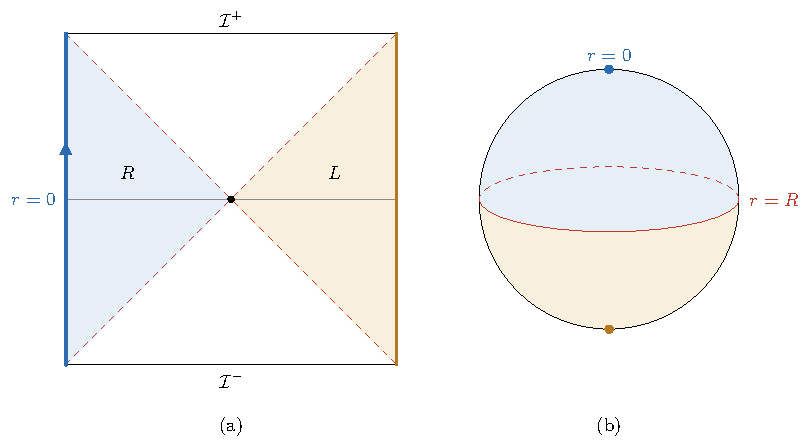
\includegraphics[width=0.82\textwidth]{figs/fig_desitter.pdf}
\caption{(a) Penrose diagram of global de~Sitter space. The left edge is the worldline of a static observer at the north pole $r=0$ (blue arrow); the cosmological horizons (dashed red diagonals) confine everything this observer can ever see to the static patch $R$ (blue), while the patch $L$ (gold) belongs to an observer at the south pole (right edge). The top and bottom edges are future and past infinity $\mathcal I^\pm$, and the gray line is the $t=0$ slice. (b) That slice is a sphere: its northern half (blue) lies in $R$ and ends on the horizon $r=R$ (red equator), which is the black dot in (a).}
\label{fig:desitter}
\end{figure}

The \emph{generalized} de~Sitter entropy, $S_{\text{gen}}=A_{\text{hor}}/4G_N+\widetilde S_R$, has a strange
feature that is the opposite of a black hole's behavior: \textbf{exciting matter in the static patch
\emph{decreases} $S_{\text{gen}}$}, because it shrinks the cosmological horizon area faster than it grows the
matter entanglement $\widetilde S_R$. This can be checked completely explicitly: put a black hole of mass
parameter $\mu$ inside the static patch (giving a black-hole horizon at $r_b$ nested inside the cosmological
horizon at $r_c>r_b$), represent $\widetilde S_R$ by the black-hole horizon area itself, and the generalized
entropy comes out to $S_{\text{gen}}=\omega_{d-2}(r_c^{d-2}+r_b^{d-2})/4G_N$, which is \emph{always less} than
$S_{\text{dS}}$ — so $S_{\text{dS}}$ is the maximum possible value of $S_{\text{gen}}$, achieved exactly by
empty de~Sitter.

\subsection*{Worked calculation: why matter excitations decrease de~Sitter entropy}

To see this thermodynamic behavior in detail, consider a four-dimensional Schwarzschild--de~Sitter spacetime
with metric:
\[
ds^2 = -f(r) dt^2 + \frac{dr^2}{f(r)} + r^2 d\Omega_2^2, \qquad f(r) = 1 - \frac{2 G_N M}{r} -
\frac{r^2}{R^2} .
\]
\begin{enumerate}
\item \textbf{Empty de~Sitter space ($M = 0$)}:
The horizon condition $f(r) = 1 - r^2/R^2 = 0$ gives a single cosmological horizon at $r_c^{(0)} = R$.
The cosmological horizon area is $A_{\text{dS}} = 4\pi R^2$, giving the Gibbons--Hawking entropy:
\[
S_{\text{dS}} = \frac{A_{\text{dS}}}{4 G_N} = \frac{\pi R^2}{G_N} .
\]
\item \textbf{Matter excitation: small black hole ($0 < G_N M \ll R$)}:
For a localized excitation of mass $M$, the horizon equation $f(r) = 0$ has two positive roots: a black hole
horizon at $r_b$ and a shifted cosmological horizon at $r_c < R$.
Let $r_c = R(1 - \delta)$ with $\delta \ll 1$. Expanding $f(r_c) = 0$ to first order in $\delta$ and $M$:
\[
1 - \frac{2 G_N M}{R} - (1 - 2\delta) \approx 0 \implies \delta = \frac{G_N M}{R} .
\]
Therefore the cosmological horizon shrinks to $r_c \approx R\left(1 - \frac{G_N M}{R}\right)$.
Its shifted area is:
\[
A_c(M) = 4\pi r_c^2 \approx 4\pi R^2 \left(1 - \frac{2 G_N M}{R}\right) = A_{\text{dS}} - 8\pi G_N M R .
\]
The black hole horizon is at $r_b \approx 2 G_N M$, with area $A_b(M) = 4\pi r_b^2 \approx 16\pi G_N^2 M^2
\sim O(G_N^2 M^2)$.
The total generalized entropy is the sum of both horizon areas:
\begin{align}
S_{\text{gen}}(M) = \frac{A_c(M)}{4 G_N} + \frac{A_b(M)}{4 G_N}
&\eqstep{1} \frac{A_{\text{dS}} - 8\pi G_N M R}{4 G_N} + O(G_N M^2) \notag\\
&\eqstep{2} S_{\text{dS}} - 2\pi M R + O(G_N M^2) . \notag
\end{align}
\stepwhy{1}{substitute the shifted cosmological area $A_c(M)=A_{\text{dS}}-8\pi G_NMR$, and note that the
black-hole term $A_b/4G_N\approx4\pi G_NM^2$ is second order in $M$.}\quad
\stepwhy{2}{split the fraction: $A_{\text{dS}}/4G_N=S_{\text{dS}}$ and $8\pi G_NMR/4G_N=2\pi MR$.}
\end{enumerate}
Here $\beta_{\text{dS}} = 2\pi R$ is the inverse Gibbons--Hawking temperature. Thus, to linear order in
perturbation:
\[
S_{\text{gen}}(M) - S_{\text{dS}} = -\beta_{\text{dS}} M < 0 \quad \text{for all } M > 0 .
\]
Any localized energy excitation inside the static patch strictly \textbf{lowers} the generalized entropy.
Consequently, empty de~Sitter ($M = 0$) is the unique state of \textbf{maximal entropy}.

\subsection*{Recognizing the type \texorpdfstring{$\mathrm{II}_1$}{II1} signature}

This behavior — a reference state whose entropy can only ever decrease under perturbation — is exactly what
appeared, worked out on an explicit example, in the type $\mathrm{II}_1$ Bell-pair chain of Chapter~3, where
perturbing away from the maximally entangled $\ket{\Phi_{\pi/4}}$ always gives $S_\M(\Psi)\le0$.
\textbf{Empty de~Sitter behaves exactly like the maximally entangled reference state of a type
$\mathrm{II}_1$ algebra, with $R$ and $L$ static patches playing the role of the two entangled halves.}

Making this precise uses exactly the observer model above, with one small but crucial modification. Take
$\HH_Q$ to be the QFT Hilbert space on global de~Sitter, $\ket\Psi$ the Bunch--Davies vacuum, $\M,\M'$ the $R$-
and $L$-patch algebras (modular Hamiltonian $K$ = the boost generator of $t$-translations), and $\hat q_R,\hat
q_L$ the Hamiltonians of static observers at the two poles. This reproduces $\widehat\M_R,\widehat\M_L$ exactly
as before — \emph{except} that now $\hat q_R,\hat q_L$ are required to be \textbf{bounded below} (non-negative
eigenvalues — physically, the sensible statement that a real observer's energy cannot be negative). By exactly
the mechanism checked in Chapter~5 (restricting the clock spectrum to $q\ge0$ turns a divergent trace into a
normalized one), $\widehat\M_R,\widehat\M_L$ become type $\mathrm{II}_1$, not type $\mathrm{II}_\infty$. The
type $\mathrm{II}_1$ entropy relative to the maximally entangled reference state
$\ket{\widehat\Psi_T}=e^{-\hat q/2}\otimes\ket0_{\text{BD}}$, with trace $\tr(\cdots)\equiv\braket{
\widehat\Psi_T|\cdots|\widehat\Psi_T}$, is negative exactly the way the Chapter~3 example was, and for the
identical reason: there is no unentangled reference to fall below zero from, only a maximally entangled one to
fall below.

One more consistency check resolves an objection that looks fatal at first glance: if empty de~Sitter is a
maximally entangled state, should it not have infinite temperature (the way a maximally entangled Bell pair
has infinite temperature in the entanglement-Hamiltonian sense)? The resolution: the state
$\ket{\widehat\Psi_T}$ has density operator $\rho=e^{-K}$ on the crossed-product algebra — a thermal state at
\emph{dimensionless} temperature exactly $1$, the universal modular temperature of Tomita--Takesaki theory
(Chapter~4). Converting this dimensionless $\beta=1$ into physical units using the static observer's own
proper time $t$ reproduces exactly the known, finite de~Sitter temperature $T_{\text{dS}}=1/2\pi R$. There is
no contradiction: ``maximally entangled'' was always a dimensionless, modular-time statement, and the finite
physical temperature only appears once you convert to an observer's physical clock.

\begin{table}[htbp]
\centering
\small
\renewcommand{\arraystretch}{1.3}
\begin{tabularx}{\textwidth}{>{\bfseries\color{navyhead}}l >{\raggedright\arraybackslash}X >{\raggedright\arraybackslash}X}
\toprule
Property & Black Hole Exterior (AdS/Minkowski) & de~Sitter Static Patch \\
\midrule
Spacetime Horizon & Event horizon (null boundary of black hole interior) & Cosmological horizon (null boundary of observer static patch) \\
Horizon Temperature & Hawking temperature $T_H = \frac{1}{8\pi G_N M}$ & Gibbons--Hawking temperature $T_{\text{dS}} = \frac{H}{2\pi} = \frac{1}{2\pi R}$ \\
Killing Vector $\chi = \partial_t$ & Timelike outside; null on horizon; timelike again at spatial infinity & Timelike inside static patch; null on cosmological horizon; spacelike outside \\
Reference Vacuum State & Hartle--Hawking vacuum $\ket{\Psi_{\text{HH}}}$ & Bunch--Davies vacuum $\ket{0_{\text{BD}}}$ \\
Clock Hamiltonian $\hat q$ & $\hat q \in (-\infty, \infty)$ (unbounded real line) & $\hat q \ge 0$ (energy bounded below for physical observer) \\
Crossed Product Algebra & Type $\mathrm{II}_\infty$ factor ($\tr(\id) = \int_{-\infty}^\infty dq\,e^{-q} = \infty$) & Type $\mathrm{II}_1$ factor ($\tr(\id) = \int_0^\infty dq\,e^{-q} = 1$) \\
Entropy Formula & $S_{\widehat\M} = -S(\Phi\|\Psi) + \text{const} = S_{\text{gen}} + \text{const}$ & $S_{\widehat\M} \le 0$ (relative to maximally entangled empty de Sitter) \\
Perturbation Response & $\Delta S_{\text{gen}} > 0$ (adding matter increases horizon area) & $\Delta S_{\text{gen}} = -\beta_{\text{dS}} M < 0$ (matter shrinks cosmological horizon) \\
Maximal Entropy State & None (entropy can grow unboundedly with mass $M$) & Empty de~Sitter ($M = 0$, $S_{\text{max}} = S_{\text{dS}} = \frac{\pi R^2}{G_N}$) \\
\bottomrule
\end{tabularx}
\caption{Comprehensive algebraic and thermodynamic comparison between the black hole exterior and the de~Sitter static patch under the crossed-product construction.}
\label{tab:bh_vs_desitter}
\end{table}

\section{Application III: generalized entropy for a local spacetime region}

The black hole and de~Sitter examples both had a special simplifying feature: a single reference state existed
whose modular Hamiltonian coincided exactly with an honest geometric (isometric) time flow. A more general
region has no such flow. A standard example is Schwarzschild--de~Sitter: a black hole sitting inside a
de~Sitter universe, so the observer's accessible region is bounded by \emph{two} horizons at different
temperatures, $r_b<r_c$. With no common temperature, there is no single global geometric modular flow at all.
The construction generalizes cleanly: decompose the region's algebra as $\M_R=\M_c\otimes\M_b$ (cosmological-
and black-hole-horizon factors), choose a state making \emph{each} factor's modular flow separately geometric,
and introduce two independent pairs of observer Hamiltonians, one for each horizon, with a separate constraint
for each. The resulting type is not what naive analogy would suggest: even with both sets of observer
Hamiltonians bounded below, the algebra comes out type $\mathrm{II}_\infty$, not type $\mathrm{II}_1$ — and its
entropy reproduces exactly the expected sum of both horizon areas plus bulk matter entropy,
\[
S_{\text{gen}}=\frac{A_{\text{cos}}}{4G_N}+\frac{A_{\text{BH}}}{4G_N}+\widetilde S_R .
\]
This shows the crossed-product mechanism is robust and general, not a special property of the two simplest
(black hole, de~Sitter) examples.

\section{A model of dynamical observers}

Every model so far treated the observer's own trajectory as fixed, non-dynamical — only its clock was quantum
mechanical. A more honest model lets the observer itself be a genuine, finite-mass dynamical particle, worked
out for two-dimensional de~Sitter space: promoting the particle's mass to a dynamical variable $Q(\tau)$ with
conjugate $P(\tau)$ and gauging the full de~Sitter isometry group (rather than just time translations)
produces a richer physical Hilbert space, with gauge-invariant, ``dressed'' field operators $\phi_R$ built by
projecting onto observer-frame matrix elements. A key structural result: the resulting observer algebra
$\Alg_R$ turns out to be a direct integral of type $\mathrm{I}_\infty$ factors — because a genuinely dynamical
observer can change its own trajectory, there is no fixed subregion its dressed operators stay confined to, so
they end up smeared, state-dependently, over an entire Cauchy slice. The static-observer limit of the
de~Sitter discussion above is recovered by sending the observer's mass $\Lambda\to\infty$ — but this limit does
\emph{not} commute with taking the double commutant: take $\Lambda\to\infty$ first and you recover the emergent
type II algebra (and its Gibbons--Hawking entropy); take the double commutant first and then send
$\Lambda\to\infty$, and you get type I instead. The type II structure — and the cosmological horizon's very
existence as an entropic object — is itself an emergent, order-of-limits-dependent phenomenon.

\begin{physconnect}[: bounded-below spectra are why a Gibbs state exists at all]
The distinction running through Chapter~5 and the de~Sitter discussion above — whether the observer's clock
spectrum is bounded below decides type $\mathrm{II}_1$ versus type $\mathrm{II}_\infty$ — is exactly the same
distinction you already navigate every time you write down a partition function. An ordinary Gibbs state
$\rho=e^{-\beta H}/Z$ only exists as a normalizable density matrix if $Z=\Tr\,e^{-\beta H}$ converges, and
that convergence is exactly the statement that $H$ is bounded below: for the harmonic oscillator,
$H=\omega(n+\tfrac12)$ with $n=0,1,2,\dots$, so
\[
Z=\sum_{n=0}^\infty e^{-\beta\omega(n+1/2)}=\frac{e^{-\beta\omega/2}}{1-e^{-\beta\omega}}
\]
converges precisely because the sum is bounded below at $n=0$. This is the discrete, everyday version of the
exact integral check carried out in Chapter~5, $\int_0^\infty dq\,e^{-q}=1$ versus $\int_{-\infty}^\infty
dq\,e^{-q}=\infty$. A harmonic oscillator or a hydrogen atom has a ground state, and hence a sensible thermal
state at any temperature, \emph{because} its spectrum is bounded below; a system whose energy were unbounded
below would have no normalizable Gibbs state at any temperature. The observer models of this chapter are doing
nothing more exotic: a physical observer's clock Hamiltonian $\hat q$ is bounded below for the same reason a
real physical system's energy is — because a real system has a ground state — and it is exactly this ordinary
fact, not a new gravitational input, that produces the finite trace (type $\mathrm{II}_1$) and hence the
finite Gibbons--Hawking entropy of the cosmological horizon.
\end{physconnect}

With a large but finite observer mass, the observer's position becomes increasingly uncertain over time: an
initial position uncertainty $1/\Lambda$ grows to $\sim e^{2\pi\tau/\beta_{\text{dS}}}/\Lambda$ after proper
time $\tau$, from the exponential expansion of de~Sitter. This defines a natural \textbf{scrambling time}
$\tau_s\equiv\tfrac{\beta_{\text{dS}}}{2\pi}\log\Lambda$, after which the observer has an $O(1)$ chance of
leaving its original static patch. This scrambling shows up concretely in an out-of-time-order correlator (a
standard chaos diagnostic): even though the matter field itself is free and does not directly interact with
the observer, the gravitational constraint couples them nontrivially — inserting an operator along the
observer's worldline physically ``kicks'' its trajectory, and this recoil produces genuine quantum chaotic
behavior, with a decay rate matching a Lyapunov exponent of $4\pi/\beta_{\text{dS}}$ — twice the universal
chaos bound, matching a mechanism identified independently in other contexts.

\section{Operator algebras of JT gravity}

The chapter closes with a remarkable exact result, in a setting simple enough to solve completely rather than
only perturbatively: \textbf{Jackiw--Teitelboim (JT) gravity}, a two-dimensional gravity theory (with a scalar
``dilaton'' field $\Phi$) coupled to matter, whose gravitational sector reduces entirely to boundary dynamics
once the dilaton's own equation of motion is solved, forcing the bulk geometry to be locally exact AdS$_2$.
The theory's gauge freedom (the isometry group of AdS$_2$) locks the two boundaries' Hamiltonians together,
$H_L=H_R\equiv H$, reducing the classical phase space to just two variables — equivalently, the boundary
geodesic separation $\ell$ and its conjugate momentum — which can be canonically quantized into a Hilbert space
$L^2(\mathbb R)$, with an (overcomplete) basis of states $\ket\beta$, $\beta\in\mathbb R_{>0}$, built from a
Euclidean path integral. Including matter fields (which do not couple directly to the dilaton), the full
quantum-gravitational Hilbert space becomes $\HH=L^2(\mathbb R)\otimes\HH_{\text{matt}}$, with a basis built
from path integrals with matter insertions on the Euclidean boundary.

This is one of the very few places in the entire subject where ``the operator algebra of quantum gravity'' is
known in exact, closed form: the full algebra of gauge-invariant JT-gravity observables (built including the
boundary Hamiltonian $H_R$ itself, at genuinely finite $G_N$ — with no crossed product, no auxiliary observer,
and no perturbative expansion needed as an approximation) is \textbf{type II}. This result is stated here
without proof. Unlike every earlier example in this chapter, it is not a statement about a semiclassical,
large-$N$ construction dressed onto an auxiliary clock; it is an exact statement about the full
quantum-gravitational theory itself, at finite coupling. It stands as concrete proof of principle that ``the
algebra of quantum gravity,'' at finite $G_N$, is a well-posed and answerable question — not merely a
semiclassical approximation scheme — at least in this simplest of solvable models.

\bigskip
\noindent The concrete applications of this chapter — black hole, de~Sitter, Schwarzschild--de~Sitter,
dynamical observers, and exact JT gravity — are all built from the same single mechanism: gravitational
dressing to a physical observer is the crossed product by the modular group, and it is this, and nothing more
exotic, that converts an intractable type $\mathrm{III}_1$ algebra with no entropy into a genuine type II
algebra whose entropy is exactly the gravitational entropy physicists already knew to expect. Chapter~10
closes with a summary and some more speculative remarks on what all of this might mean for the mathematical
structure of quantum gravity at finite $G_N$.
